\documentclass[tikz,border=2pt]{standalone}

\usepackage{amsmath}
\usepackage{newtxtext}
\usepackage{xcolor}
\usepackage{tikz}
\usetikzlibrary{arrows.meta,positioning,fit,backgrounds,calc,decorations.pathreplacing,patterns,shapes.geometric}
\usepackage{pgfplots}
\pgfplotsset{compat=1.18}
\usepgfplotslibrary{groupplots,fillbetween}

\definecolor{bestcolor}{HTML}{E8F5E9}
\definecolor{gaincolor}{HTML}{1B5E20}
\definecolor{cStandard}{HTML}{BF616A}
\definecolor{cAOI}{HTML}{5E81AC}
\definecolor{cDelta}{HTML}{A3BE8C}
\definecolor{cVisual}{HTML}{D08770}
\definecolor{cASR}{HTML}{B48EAD}
\definecolor{cNarr}{HTML}{88C0D0}
\definecolor{cAccent}{HTML}{EBCB8B}
\definecolor{cGray}{HTML}{4C566A}
\definecolor{cLightGray}{HTML}{D8DEE9}

\begin{document}
\newcommand{\figfont}{\fontsize{7.5}{9}\selectfont}
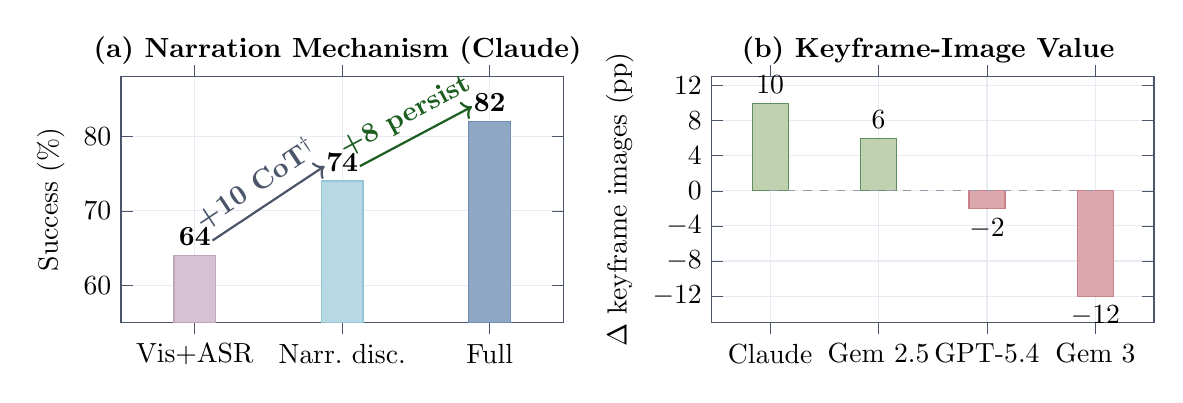
\begin{tikzpicture}
\begin{scope}[yshift=0cm]
\node[font=\figfont\bfseries, anchor=north] at (2.75,3.75) {(a) Narration Mechanism (Claude)};
\begin{axis}[
    width=7.2cm, height=4.7cm, ybar, bar width=15pt,
    ymin=55, ymax=88, ylabel={Success (\%)}, ylabel style={font=\figfont},
    xmin=0.5, xmax=3.5,
    xtick={1,2,3},
    xticklabels={Vis+ASR, Narr.\ disc., Full},
    xticklabel style={font=\figfont},
    ytick={60,70,80}, yticklabel style={font=\figfont},
    grid=major, major grid style={cLightGray!60},
    axis line style={cGray}, tick style={cGray},
    every axis plot/.append style={bar shift=0pt},
]
\addplot[fill=cASR!55,draw=cASR!80] coordinates {(1,64)};
\addplot[fill=cNarr!60,draw=cNarr!90] coordinates {(2,74)};
\addplot[fill=cAOI!70,draw=cAOI!90] coordinates {(3,82)};
\node[font=\figfont\bfseries, anchor=south] at (axis cs:1,64) {64};
\node[font=\figfont\bfseries, anchor=south] at (axis cs:2,74) {74};
\node[font=\figfont\bfseries, anchor=south] at (axis cs:3,82) {82};
\draw[->,thick,cGray] (axis cs:1.12,66) -- (axis cs:1.88,76)
  node[midway,above,font=\figfont\bfseries,text=cGray,sloped]{+10 CoT$^\dagger$};
\draw[->,thick,gaincolor] (axis cs:2.12,76) -- (axis cs:2.88,84)
  node[midway,above,font=\figfont\bfseries,text=gaincolor,sloped]{+8 persist};
\end{axis}
\end{scope}
\begin{scope}[xshift=7.5cm]
\node[font=\figfont\bfseries, anchor=north] at (2.75,3.75) {(b) Keyframe-Image Value};
\begin{axis}[
    width=7.2cm, height=4.7cm, ybar, bar width=13pt,
    ymin=-15, ymax=13, ylabel={$\Delta$ keyframe images (pp)}, ylabel style={font=\figfont},
    symbolic x coords={Claude, Gemini 2.5, GPT-5.4, Gemini 3},
    xtick={Claude, Gemini 2.5, GPT-5.4, Gemini 3},
    xticklabels={Claude, Gem 2.5, GPT-5.4, Gem 3},
    xticklabel style={font=\figfont},
    ytick={-12,-8,-4,0,4,8,12}, yticklabel style={font=\figfont},
    grid=major, major grid style={cLightGray!60},
    axis line style={cGray}, tick style={cGray}, enlarge x limits=0.18,
    nodes near coords, nodes near coords style={font=\figfont\bfseries},
    nodes near coords align={vertical},
    every axis plot/.append style={bar shift=0pt},
]
\addplot[draw=gaincolor!70,fill=cDelta!70] coordinates {(Claude,10) (Gemini 2.5,6)};
\addplot[draw=cStandard!80,fill=cStandard!55] coordinates {(GPT-5.4,-2) (Gemini 3,-12)};
\draw[cGray!60,dashed] (axis cs:Claude,0) -- (axis cs:Gemini 3,0);
\end{axis}
\end{scope}
\end{tikzpicture}
\end{document}
